\documentclass[11pt, twoside, a4paper]{book}

\usepackage{graphicx}
\usepackage[utf8]{inputenc}
\usepackage{ngerman}
%\usepackage{lineno}
\usepackage{verbatim}
\usepackage[squaren]{SIunits}
\usepackage{amsmath}
\usepackage{amsfonts}
\usepackage{amssymb}
\usepackage{enumitem}
\usepackage{fancyhdr}
\usepackage{textcomp}
\usepackage{subcaption}
\usepackage[noadjust]{marginnote}
\usepackage{tikz}
\usepackage{nicefrac}
\usepackage{framed}
\usepackage{import}

\usetikzlibrary{calc,intersections}
\usetikzlibrary{arrows}
\usetikzlibrary{decorations.markings}
\usetikzlibrary{decorations.pathreplacing}
\usepackage[european resistors]{circuitikz}
\usepackage[ 
    top=2cm, 
    bottom=2cm, 
    outer=3cm, 
    inner=3cm,
    marginparwidth=2.5cm,
		headheight=14pt
  ]{geometry}

\usepackage{parskip}
\usepackage{pdfpages}

\setlength{\parindent}{0pt}

\newcommand{\experimentheader}[4]
{
  \iftutor{{\bf Schwierigkeitsgrad:} #1\\}
  \iftutor{{\bf Dauer:} #2\\}
  {\bf Ger\"ate:} #3\\
  {\bf Bauteile:} #4
}

\newcommand{\hintboxNone}{0}
\newcommand{\hintboxExclamation}{1}
\newenvironment{hintbox}[4][\hsize]
{
  \def\FrameCommand
  {%
    {\color{#3}\vrule width 3pt}%
    \hspace{0pt}%must no space.
    \fboxsep=\FrameSep\colorbox{#4}%
  }%
  \MakeFramed{\hsize#1\advance\hsize-\width\FrameRestore}%
  \mbox{\textbf{#2}:}%
}
{
  \endMakeFramed
}
\newcommand{\xhintbox}[3]
{
  \begin{hintbox}{Achtung}{red!50}{red!10}
    #3
  \end{hintbox}
}

\newenvironment{hint}
{
  \begin{hintbox}{Hinweis}{green!50}{green!10}
}
{
  \end{hintbox}
}

\newenvironment{definition}
{
  \begin{hintbox}{Definition\\}{white!50}{white!10}
}
{
  \end{hintbox}
}

\newenvironment{important}
{
  \begin{hintbox}{Hinweis}{gray!50}{gray!10}
}
{
  \end{hintbox}
}

\newenvironment{jason}
{
  \begin{hintbox}{Achtung}{red!50}{red!10}
}
{
  \end{hintbox}
}

\newcommand{\mandatoryenumi}
{
  \renewcommand{\labelenumi}{\arabic{enumi}.} 
}
\newcommand{\optionalenumi}
{
  \renewcommand{\labelenumi}{$\bigstar$\quad\arabic{enumi}.} 
}
\newcommand{\mandatoryenumii}
{
  \renewcommand{\labelenumii}{(\alph{enumii})} 
}
\newcommand{\optionalenumii}
{
  \renewcommand{\labelenumii}{$\bigstar$\quad(\alph{enumii})} 
}
\newcommand{\icname}[1]{\mbox{\tt #1}}


  %\newcommand{\iftutor}[1]{}
\newcommand{\ifnotutor}[1]{#1}

  \newcommand{\iftutor}[1]{#1}
\newcommand{\ifnotutor}[1]{}


\newenvironment{tutorhint}{\comment}{\endcomment}
\newenvironment{todo}{\comment}{\endcomment}
\newenvironment{solution}{\comment}{\endcomment}
\iftutor
{
  \renewenvironment{todo}
  {
    \hintbox{Todo}{red!50!yellow!90}{red!50!yellow!20}
  }
  {
    \endhintbox
  }
  \renewenvironment{tutorhint}
  {
    \hintbox{Tutorenhinweis der Stunde}{blue!50}{blue!10}
  }
  {
    \endhintbox
  }
  \renewenvironment{solution}
  {
    \hintbox{L\"osung}{black!80}{black!5}
  }
  {
    \endhintbox
  }
}
\newcommand{\etutorhint}[1]
{
  \iftutor{
    \tutorhint
      #1
    \endtutorhint
  }
}
\newcommand{\esolution}[1]
{
  \iftutor
  {
    \solution
    #1
    \endsolution
  }
}
\newcommand{\etodo}[1]
{
  \iftutor
  {
    \todo
    #1
    \endtodo
  }
}



\begin{document}

\renewcommand{\thechapter}{\arabic{chapter}}
\setcounter{chapter}{9}
\def\chaptername{Versuch}

\chapter{Mikroskop}
\label{v:8}

Der Versuch erklärt die Funktionsweise des Lichtmikroskops, indem er die Beobachtung des reellen Zwischenbildes und des virtuellen Gesamtbildes ermöglicht. Auch das Grössenverhältnis von Bild und Gegenstand kann vermessen werden.

%------------------------------------------------
\section{Stichworte}
%------------------------------------------------

Reelles und virtuelles Bild; Vergrösserung; Okular, Objektiv; Numerische Apertur; Auflösungsvermögen.
%
%------------------------------------------------
\section{Literatur}
%------------------------------------------------

Gehrtsen, Kapitel 9.1.1/2, 9.2.4 bis 9.2.6 und 10.1.5
%
%------------------------------------------------
\section{Theoretischer Hintergrund}
%------------------------------------------------

Beim Mikroskop multiplizieren sich die Wirkungen zweier Linsen oder Linsensysteme. Das \textit{Objektiv} erzeugt ein möglichst großes reelles Zwischenbild des gut beleuchteten Gegenstandes. Im Prinzip könnte man schon dieses Bild beliebig groß machen, indem man den Gegenstand immer näher an die Brennebene der Objektivlinse rückt, was jedoch einige Nachteile hat:
\begin{itemize}
	\item Je größer das Zwischenbild wird, desto lichtärmer wird es. Damit wird es, selbst im dunklen Tubus des Mikroskops schwer zu erkennen.
	%
	\item Nach Gleichung \ref{eq:Abbildungsmassstab-Linse} wird bei gegebener Gegenstandsweite $g$ und -größe $G$ für eine große Bildgröße $B$ die Bildweite $b = t$, und damit die Länge des Tubus' $t$ sehr groß, was die Handhabung sehr unbequem macht.
	%
	\item Die Abbildungsfehler (sphärische und chromatische Aberration, Astigmatismus) werden größer.
	%
%	\item Durch das begrenzte Auflösungsvermögen
\end{itemize}
Der Gegenstand liegt also ganz knapp außerhalb der Objektivbrennweite $f_1$, so dass für den Abbildungsmaßstab gilt:
\begin{equation}
	\beta = \frac{B}{G} = \frac{b}{g} = \frac{t}{f_1}
\end{equation}
Offenbar muss also das Objektiv eine kleine Brennweite haben, damit das Zwischenbild groß wird. Hier liegt auch der Unterschied zum Teleskop, welches eine große Objektivbrennweite hat (Wieso?).

Dieses Zwischenbild betrachtet man mit dem \textit{Okular} als Lupe und erzielt somit eine nochmalige Vergrößerung $V_{ok}=s_0/f_2$, wobei $s_0~=~25$~cm der Abstand eines Gegenstandes vom Auge ist, bei dem man diesen mit entspanntem Auge noch scharf sehen kann. Das Zwischenbild muss dazu um die Brennweite $f_2$ hinter dem Okular sitzen.

Die Gesamtvergrößerung des Mikroskops ergibt sich aus dem Abbildungsmaßstab des Objektivs multipliziert mit der Lupenvergrößerung des Okulars zu
\begin{equation}
	V_{ges} = \frac{B}{G} = \frac{t}{f_1} \frac{s_0}{f_2}
\label{eq:Vergoesserung_Mikroskop}
\end{equation}

\subsection{Das Auflösungsvermögen optischer Geräte}

Jede Linse, begrenzt durch ihren Rand oder ihre Fassung, wirkt als beugende Öffnung (vgl. Versuch \ref{v:10}). Das bedeutet, dass sie auch von einem unendlich weit entfernten Punkt (z. Bsp. einem Stern) keinen absolut scharfen Bildpunkt erzeugt, sondern vielmehr ein \textit{Beugungsbild}. Die Breite des \textit{Hauptmaximums} der Intensität des Beugungsbildes hat einen Winkeldurchmesser von $1,22\frac{\lambda}{r}$, mit dem Radius $r$ der Linse. Zwei nahe beieinanderstehende Sterne lassen sich im Fernrohr nur als zwei getrennte Objekte erkennen, wenn ihre Beugungsscheibchen sich nicht überdecken.

Beim Mikroskop ist das Licht, das durch das Objektiv fällt, natürlich nicht parallel. Betrachtet man als Objekt einen hellen Punkt, so hat das Büschel der Lichtstrahlen, die durch das Objektiv treten einen Öffnungswinkel $\varphi$ mit der \textit{numerischen Apertur}
\begin{equation} \label{eq:num-Apertur}
	\sin\varphi = \frac{r}{f}\, ,
\end{equation} 
mit dem Radius $r$ der Objekivblende und dem Abstand $f$ zwischen Objekt und Objektiv, welcher ja fast gleich der Brennweite des Objektivs ist.\\
Der leuchtende Punkt erzeugt in der Zwischenbildebene ein Beugungsscheibchen mit einem Öffnungswinkel von $1,22\frac{\lambda}{r}$. Ein anderer leuchtender Punkt muss also mindestens um diesen Winkel, d.h. in der Objektebene um den Abstand $x_{min}~=~1,22f\lambda/r$ davon entfernt sein, damit die Scheibchen nicht verschmelzen. Mit der numerischen Apertur (s. Gleichung \ref{eq:num-Apertur}) kann man auch schreiben
%
\begin{equation}
	x_{min} \approx \frac{\lambda}{\sin\varphi}\, .
\end{equation}
%
Ein Mikroskop löst also umso besser auf, je kleiner die Wellenlänge $\lambda$ und je größer $\varphi$ ist.\\
Um die Vergrößerung kurzbrennweitiger Objektive auszunutzen, bringt man zwischen Objekt und Objektiv ein brechendes Medium (Immersionsöl), das die Wellenlänge auf $\lambda/n$ verringert. Dann ist
%
\begin{equation}
	x_{min} = \frac{\lambda}{n\,\sin\varphi} \, ,
\end{equation}
%
die numerische Apertur vergrößert sich auf $n\,\sin\varphi$.

Diese \textit{Beugungsbegrenzung} des Auflösungsvermögens wird als \textit{Auflösungsbegrenzung} oder \textit{Abbe-Limit} bezeichnet, nach Ernst Abbe, der diese Beziehung im 19. Jahrhundert beschrieb. Neuere Mikroskopieverfahren erreichen Auflösungen, die wesentlich unter diesem Abbe-Limit liegen, indem sie Details eines Präparates, die zu dicht nebeneinanderliegen, um optisch aufgelöst zu werden, nacheinander aufnehmen und das gesamte Bild im Nachhinein wieder zusammensetzen\footnote{Z. Bsp. Nobelpreis für Chemie, 2014, Stefan Hell zusammen mit Eric Betzig und William E. Moerner „for the development of super-resolved fluorescence microscopy“}. Dies bedeutet jedoch auf keinen Fall, dass das Abbe-Limit nicht mehr gilt, wie man manchmal hört. Vielmehr wird es nur in cleverer Art und Weise umgangen.

\begin{tutorhint}
%------------------------------------------------
\section{Fragen zur Vorbereitung}
%------------------------------------------------

\begin{enumerate}
 %
 \item Was soll heute im Praktikum gemessen werden? Warum?
 %
 \item Wie ist die Vergrößerung einer Linse definiert?
 %
 \item Aus welchen Teilen ist ein optisches Mikroskop aufgebaut ? (kein Strahlengang)
 %
 \item Wieso macht man nicht schon das Zwischenbild sehr groß indem man den Gegenstand immer näher an die Brennebene des Objektivs heranrückt? Welche Probleme würden auftreten?
 % 1. Zwischenbild wird lichtschwächer
 % 2. Tubuslänge immer größer
 % 3. wachsende Abbildungsfehler
 % 4. beschränktes Auflösungsvermögen erlaubt nicht beliebig kleine Einzelheiten zu erkennen
 %
 \item Beschreiben Sie das Prinzip eines Elektronenmikroskops.
 %
 \item Beschreiben Sie das Prinzip eines Raster Tunnelmikroskops (RTM).
 %
 \item Konstruieren Sie den Strahlengang an der Lupe.
 %
 \item Konstruieren Sie den Strahlengang im Mikroskop. Was ist beim Fernrohr anders?
%
\end{enumerate}
\end{tutorhint}

%------------------------------------------------
\section{Durchführung} 
%------------------------------------------------




\begin{enumerate}
 %
\begin{minipage}{0.5\textwidth}
 \item Messung der Gesamtvergrößerung $V_{ges}$ des Mikroskops:\\
  Betrachten Sie mit einem Auge einen Gegenstand $G$ (Objektmaßstab) bekannter Größe. Vergleichen Sie das Bild mit einem Maßstab $B$, der mit dem zweiten Auge neben dem Mikroskop zu sehen ist. Das Größenverhältnis von $B$ zu $G$ liefert die Vergrößerung:
  \[
  V_{ges} = \frac{B}{G}
  \]
  Wiederholen Sie die Messung drei Mal.
	%
	\item Messung der Objektivvergrößerung $V_{obj}$:\\
  Stellen Sie das Mikroskop so ein, dass der Objektmaßstab scharf abgebildet wird. Ändern Sie diese Einstellung danach nicht mehr!\\
\end{minipage}
%
\begin{minipage}{0.5\textwidth}
	\centering
		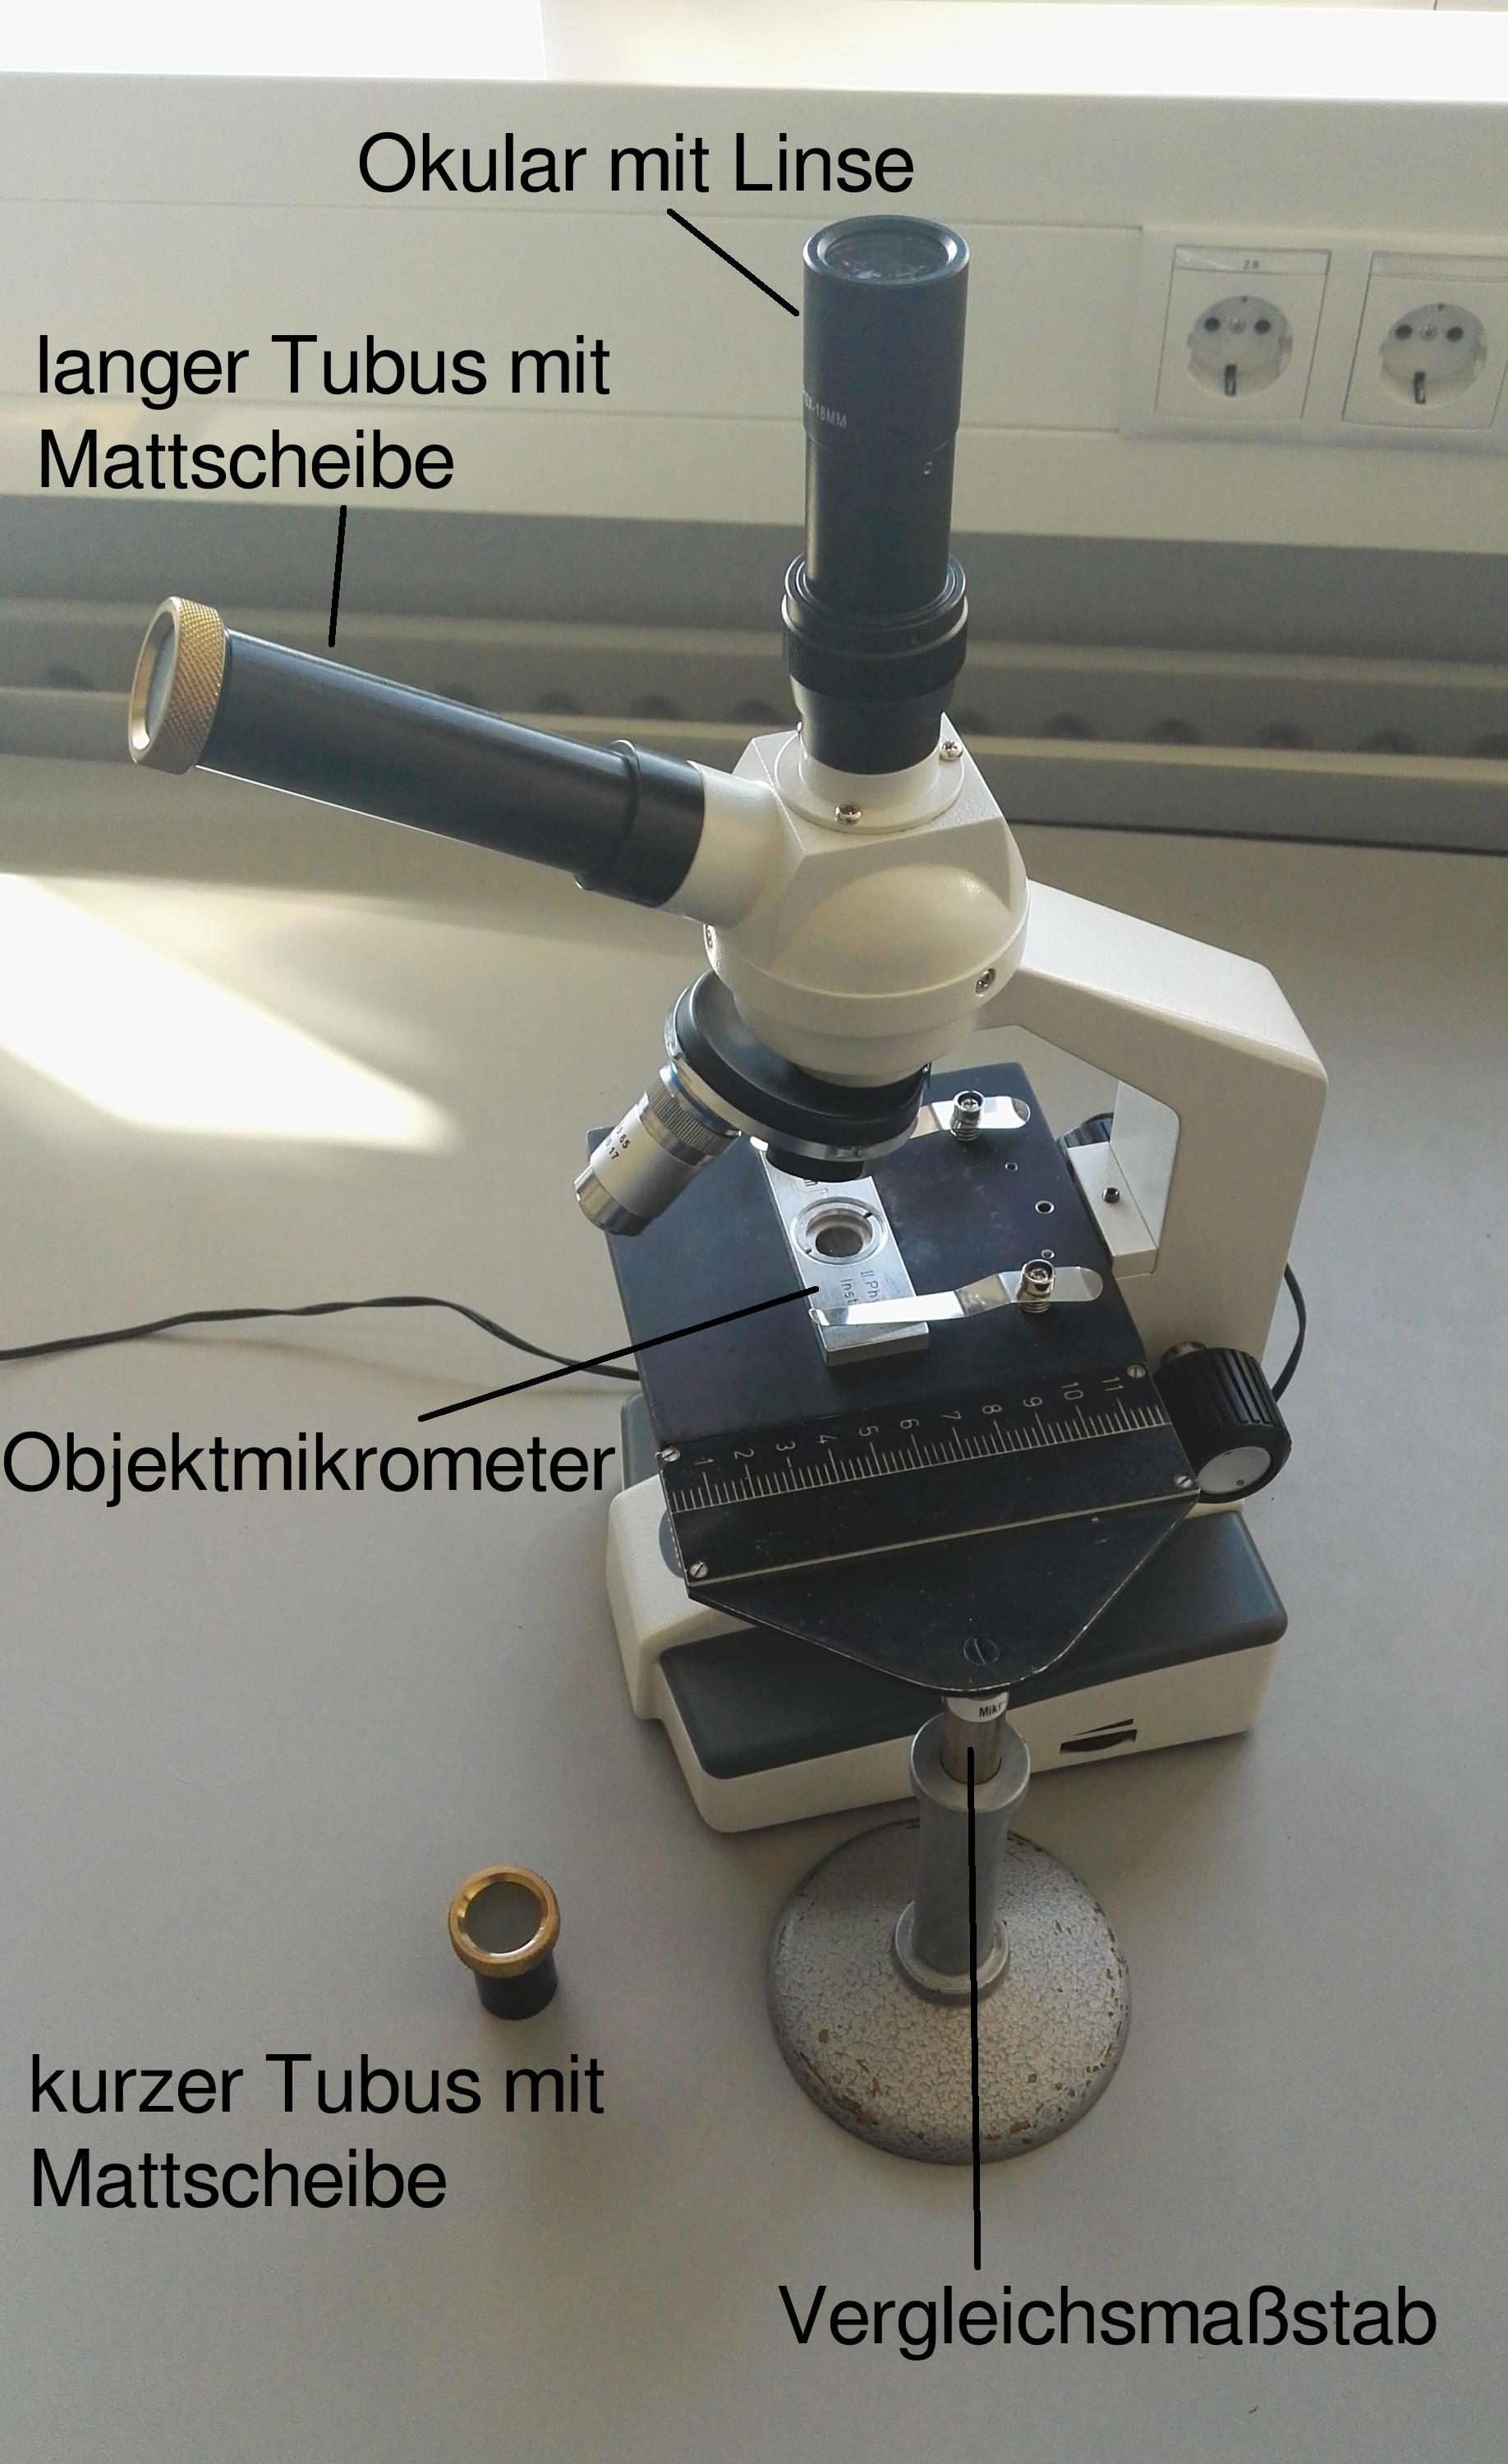
\includegraphics[width=0.7\textwidth]{Abbildungen/mikroskopbildA.jpg}
	\label{fig:mikroskopbildA}
\end{minipage}
 
	Benutzen Sie nun das geneigte Okular mit dem kurzen verschiebbaren Tubus mit Mattscheibe. Verschieben Sie die Mattscheibe, bis das reele Zwischenbild scharf ist. Hierzu verdunkeln Sie am besten den Raum. Messen Sie die Größe des Zwischenbildes, $B_Z$, mit der Schieblehre. Die Objektivvergrößerung ergibt sich nach:
  \[
  V_{obj} = \frac{B_Z}{G}
  \]
  Wiederholen Sie die Messung drei Mal.
 %
 \item Bestimmung der Objektivbrennweite $f_{obj}$:\\
  Benutzen Sie das Objektiv als Sammellinse und messen Sie die Größe des Zwischenbildes $B_Z$ für zwei Scharfeinstellungen auf der Mattscheibe:
  \begin{enumerate}
   \item mit dem kurzen Tubus: Setzen Sie den kurzen verschiebbaren Tubus mit Mattscheibe ein und messen Sie die Zwischenbildgröße $B_Z^{kurz}$ nachdem Sie das Bild scharf gestellt haben.
    \[
     V_{kurz} = \frac{B_Z^{kurz}}{G}
    \]
   %
   \item mit dem langen Tubus: Setzen Sie nun den langen Tubus mit Mattscheibe ein und messen Sie die Zwischenbildgröße $B_Z^{lang}$ nach erneuter Scharfstellung.
    \[
     V_{lang} = \frac{B_Z^{lang}}{G}
    \]
   %
   \item Messen Sie die Tubuslängen $t_1$ und $t_2$.
  \end{enumerate}
 %
 \item Bestimmung der Dicke eines Haares:\\
  Setzen Sie den kurzen verschiebbaren Tubus mit Mattscheibe ein und messen Sie die Zwischenbildgröße eines Haares mit der Schieblehre. 
\end{enumerate}

%------------------------------------------------
\section{Auswertung} 
%------------------------------------------------
\etodo{Musterauswertung}
\begin{enumerate}
%
\item Zeichnen Sie den Strahlengang im Mikroskop. Beschriften sie alle Brennpunkte, Gegenstands- und Bildgröße sowie die dazugehörige Gegenstands- und Bildweite.\\
Tip: Nutzen sie zur Konstruktion des Strahlengangs nur Parallel- bzw. Brennpunkt- und Mittelpunkstrahlen.
%
\item Berechnen Sie aus der Gesamtvergrößerung $V_{ges} = V_{obj}\cdot V_{ok}$ nun die Okularvergrößerung.\\
Berechnen sie die Fehler $\Delta V_{ges}$ und $\Delta V_{obj}$ über die Standardabweichung des Mittelwerts. Berechnen sie nun $\Delta V_{ok}$ mithilfe der Fehlerfortpflanzung. Leiten sie die dafür nötigen Ableitungen explizit her!
%
\item Berechnen Sie die Brennweite des Objektivs mit:
\begin{equation*}
f_{obj} = \left(t_2-t_1\right)\cdot\left(V_{lang}- V_{kurz}\right)
\end{equation*}
Berechnen Sie den Fehler auf die Brennweite.
%
\item Berechnen Sie die Dicke des Haares mithilfe der gemessenen Vergrößerung $V_{kurz}$.
%
\item Diskutieren sie entscheidende Fehlerquellen in diesem Versuch.
%
\end{enumerate}

\end{document}